% https://github.com/jgm/pandoc-templates/blob/master/default.latex
% http://rmarkdown.rstudio.com/pdf_document_format.html#custom_templates

\documentclass[12pt, oneside]{book}
\usepackage{lmodern}
\usepackage{amssymb,amsmath}
\usepackage{ifxetex,ifluatex}
\usepackage{fixltx2e} % provides \textsubscript
\ifnum 0\ifxetex 1\fi\ifluatex 1\fi=0 % if pdftex
  \usepackage[T1]{fontenc}
  \usepackage[utf8]{inputenc}
\else % if luatex or xelatex
  \usepackage{unicode-math}
  \defaultfontfeatures{Ligatures=TeX,Scale=MatchLowercase}
\fi
% use upquote if available, for straight quotes in verbatim environments
\IfFileExists{upquote.sty}{\usepackage{upquote}}{}
% use microtype if available
\IfFileExists{microtype.sty}{%
\usepackage[]{microtype}
\UseMicrotypeSet[protrusion]{basicmath} % disable protrusion for tt fonts
}{}
\PassOptionsToPackage{hyphens}{url} % url is loaded by hyperref
\usepackage[unicode=true]{hyperref}
\hypersetup{
            pdftitle={A Study in Disaster},
            pdfauthor={mauveSushi},
            pdfborder={0 0 0},
            breaklinks=true}
\urlstyle{same}  % don't use monospace font for urls





%%%%%%%%%%%%%%%%%%%%%%%%%%%%%%%%%%%%%%%%%%%%%%%%%%%%%
% CUSTOM
%%%%%%%%%%%%%%%%%%%%%%%%%%%%%%%%%%%%%%%%%%%%%%%%%%%%%

% margin
\usepackage[letterpaper, margin=1in]{geometry}
\usepackage{titlesec}
% change "Chapter" prefix in a book to "Section"

% hide chapter text
\renewcommand{\chaptername}{Section}
\titleformat{\chapter}{\normalfont\huge\bf}{\thechapter.}{20pt}{\huge\bf}

% title page style
\newcommand*{\titleGM}{\begingroup % Create the command for including the title page in the document
\hbox{ % Horizontal box
\hspace*{0.2\textwidth} % Whitespace to the left of the title page
\rule{1pt}{\textheight} % Vertical line
\hspace*{0.05\textwidth} % Whitespace between the vertical line and title page text
\parbox[b]{0.75\textwidth}{ % Paragraph box which restricts text to less than the width of the page
  {\noindent\Huge\bfseries A Study in Disaster}\\[2\baselineskip] % Title
  {\large \textit{The Titanic Survivors}}\\[4\baselineskip] % Tagline or further description
  {\Large \textsc{mauveSushi}} % Author name

  \vspace{0.5\textheight} % Whitespace between the title block and the publisher
  {\noindent\large Skidmore College}\\[\baselineskip] % Publisher and logo
  }
}
\endgroup}

%%%%%%%%%%%%%%%%%%%%%%%%%%%%%%%%%%%%%%%%%%%%%%%%%%%%%






\usepackage{natbib}
\bibliographystyle{apalike}
\usepackage{longtable,booktabs}
% Fix footnotes in tables (requires footnote package)
\IfFileExists{footnote.sty}{\usepackage{footnote}\makesavenoteenv{long table}}{}
\usepackage{graphicx,grffile}
\makeatletter
\def\maxwidth{\ifdim\Gin@nat@width>\linewidth\linewidth\else\Gin@nat@width\fi}
\def\maxheight{\ifdim\Gin@nat@height>\textheight\textheight\else\Gin@nat@height\fi}
\makeatother
% Scale images if necessary, so that they will not overflow the page
% margins by default, and it is still possible to overwrite the defaults
% using explicit options in \includegraphics[width, height, ...]{}
\setkeys{Gin}{width=\maxwidth,height=\maxheight,keepaspectratio}
\IfFileExists{parskip.sty}{%
\usepackage{parskip}
}{% else
\setlength{\parindent}{0pt}
\setlength{\parskip}{6pt plus 2pt minus 1pt}
}
\setlength{\emergencystretch}{3em}  % prevent overfull lines
\providecommand{\tightlist}{%
  \setlength{\itemsep}{0pt}\setlength{\parskip}{0pt}}
\setcounter{secnumdepth}{5}
% Redefines (sub)paragraphs to behave more like sections
\ifx\paragraph\undefined\else
\let\oldparagraph\paragraph
\renewcommand{\paragraph}[1]{\oldparagraph{#1}\mbox{}}
\fi
\ifx\subparagraph\undefined\else
\let\oldsubparagraph\subparagraph
\renewcommand{\subparagraph}[1]{\oldsubparagraph{#1}\mbox{}}
\fi

% set default figure placement to htbp
\makeatletter
\def\fps@figure{htbp}
\makeatother

\usepackage{booktabs}
\usepackage{longtable}
\usepackage{hyperref}
\usepackage{amsthm}
\usepackage[dvipsnames,table,xcdraw]{xcolor}
\usepackage[breakable, theorems, skins]{tcolorbox}

% color palette
\definecolor{Azure}{rgb}{0.0, 0.5, 1.0}

\makeatletter
% adjust theorem spacing
\def\thm@space@setup{%
  \thm@preskip=8pt plus 2pt minus 4pt
  \thm@postskip=\thm@preskip
}

% colorie hyperlink
\hypersetup{
    colorlinks=true,
    citecolor={black},
    linkcolor={black},
    menucolor={black},
    urlcolor={Azure}
}

% make function greybox
\DeclareRobustCommand{\greybox}[2][gray!10]{%
\begin{tcolorbox}[   %% Adjust the following parameters at will.
        breakable,
        left=0pt,
        right=0pt,
        top=0pt,
        bottom=0pt,
        colback=#1,
        colframe=#1,
        width=\dimexpr\textwidth\relax, 
        enlarge left by=0mm,
        boxsep=5pt,
        arc=0pt,outer arc=0pt,
        ]
        #2
\end{tcolorbox}
}

\makeatother

\title{A Study in Disaster}
\author{mauveSushi}
\date{2017-12-11}



%%%%%%%%%%%%%%%%%%%%%%%%%%%%%%%%%%%%%%%%%%%%%%%%%%%%%
% DOCUMENT BEGIN
%%%%%%%%%%%%%%%%%%%%%%%%%%%%%%%%%%%%%%%%%%%%%%%%%%%%%

\begin{document}
% replace the default title page by removing \maketitle
% % \maketitle
% 
\pagestyle{empty}  % Removes page numbers need the blank line before of this line
\titleGM


\fontsize{12}{16}\selectfont

\hypertarget{abstract}{%
\chapter*{Abstract}\label{abstract}}
\addcontentsline{toc}{chapter}{Abstract}

This research aims to construct a logistic regression model to predict
the survival outcome of passenger on the Titanic based on their various
demographic and socioeconomic factors, such as age, gender, number of
spouses and siblings, passenger class, etc. The findings of this
research can be generalized to most shipwreck where the ship is
considered big (having capacity of at least 1000 passengers) and the
route is through Atlantic Ocean in the early 20\textsuperscript{th}
century. We used logistic regression in tandem with backward feature
selection to obtain several prediction models. We evaluate each obtained
model using the Hosmer-Lemeshow goodness-of-fit test and then conduct a
more vigorous feature selection process to come up with the best models.
Despite the different approaches, all of the obtained models suggest a
common trend that children, woman and first class passengers are among
the one with highest chance of survival.

\hypertarget{introduction}{%
\chapter*{Introduction}\label{introduction}}
\addcontentsline{toc}{chapter}{Introduction}

On that fateful night April 15, 1912, the great Titanic carrying 2,200
people struck an iceberg and sank, brought down with it 1,500 poor
souls. Such tragedy never fails to leave all of us unsettled, but as
statisticians, we are naturally drawn to ask ourselves the question:
\emph{``How do demographic and socioeconomic factors affect chance of
survival in disaster?''} Perhaps, based on just the titanic data set,
such general question cannot be answered, since our findings are
probably just generelizable to a specific type of disaster, which is
shipwreck and to a time-frame limited to the early
20\textsuperscript{th} century. Also, we have to consider the fact that
Titanic is not just another ship\ldots{} It is (even till today) one of
the most luxurious ship ever been built (see figure below - the ship
even had swimming pool and tennis court at the lowest level!). As such,
we think the findings we obtain using this data set can only be
generalized to big ship, i.e.~ships whose capacity is at least 1000,
crossing the Pacific ocean. Note that this number 1000 seems rather
arbitrary, but we found that nowadays, on average, cruise ships with
tonnage of around 40,000 usually have capacity of 1,000
passengers\footnote{CruiserMapper,
  \href{http://www.cruisemapper.com/wiki/761-cruise-ship-passenger-capacity-ratings}{Cruise
  Ship Passenger Capacity}} and most of the bigger ships in early
20\textsuperscript{th} century were around 40,000 or more in
tonnage\footnote{Wikipedia,
  \href{https://en.wikipedia.org/wiki/List_of_largest_passenger_ships}{List
  of largest passenger ships}}. For this reason, we formulate our
research question as follows:

\textbf{``How do various demographic and socioeconomic factors affect
chance of survival in shipwreck where the ship's capacity is at least
1000 passegners and the route is through the Atlantic Ocean in the early
20\textsuperscript{th} century?''}

In simpler words, we will attempt to create a model to be able to
predict the survival outcome of a passenger, given his/her relevant
background information. We constructed several different models with 2
major approaches, one using backward selection and one using a more
rigorous feature selection process. Despite this, the models we obtain
show a common trend that female, little kids and first-class passengers
are more likely to survive the shipwreck. Following this, we will step
by step present our data preparation and modelling process, as well as
our findings.

\begin{figure}
\centering
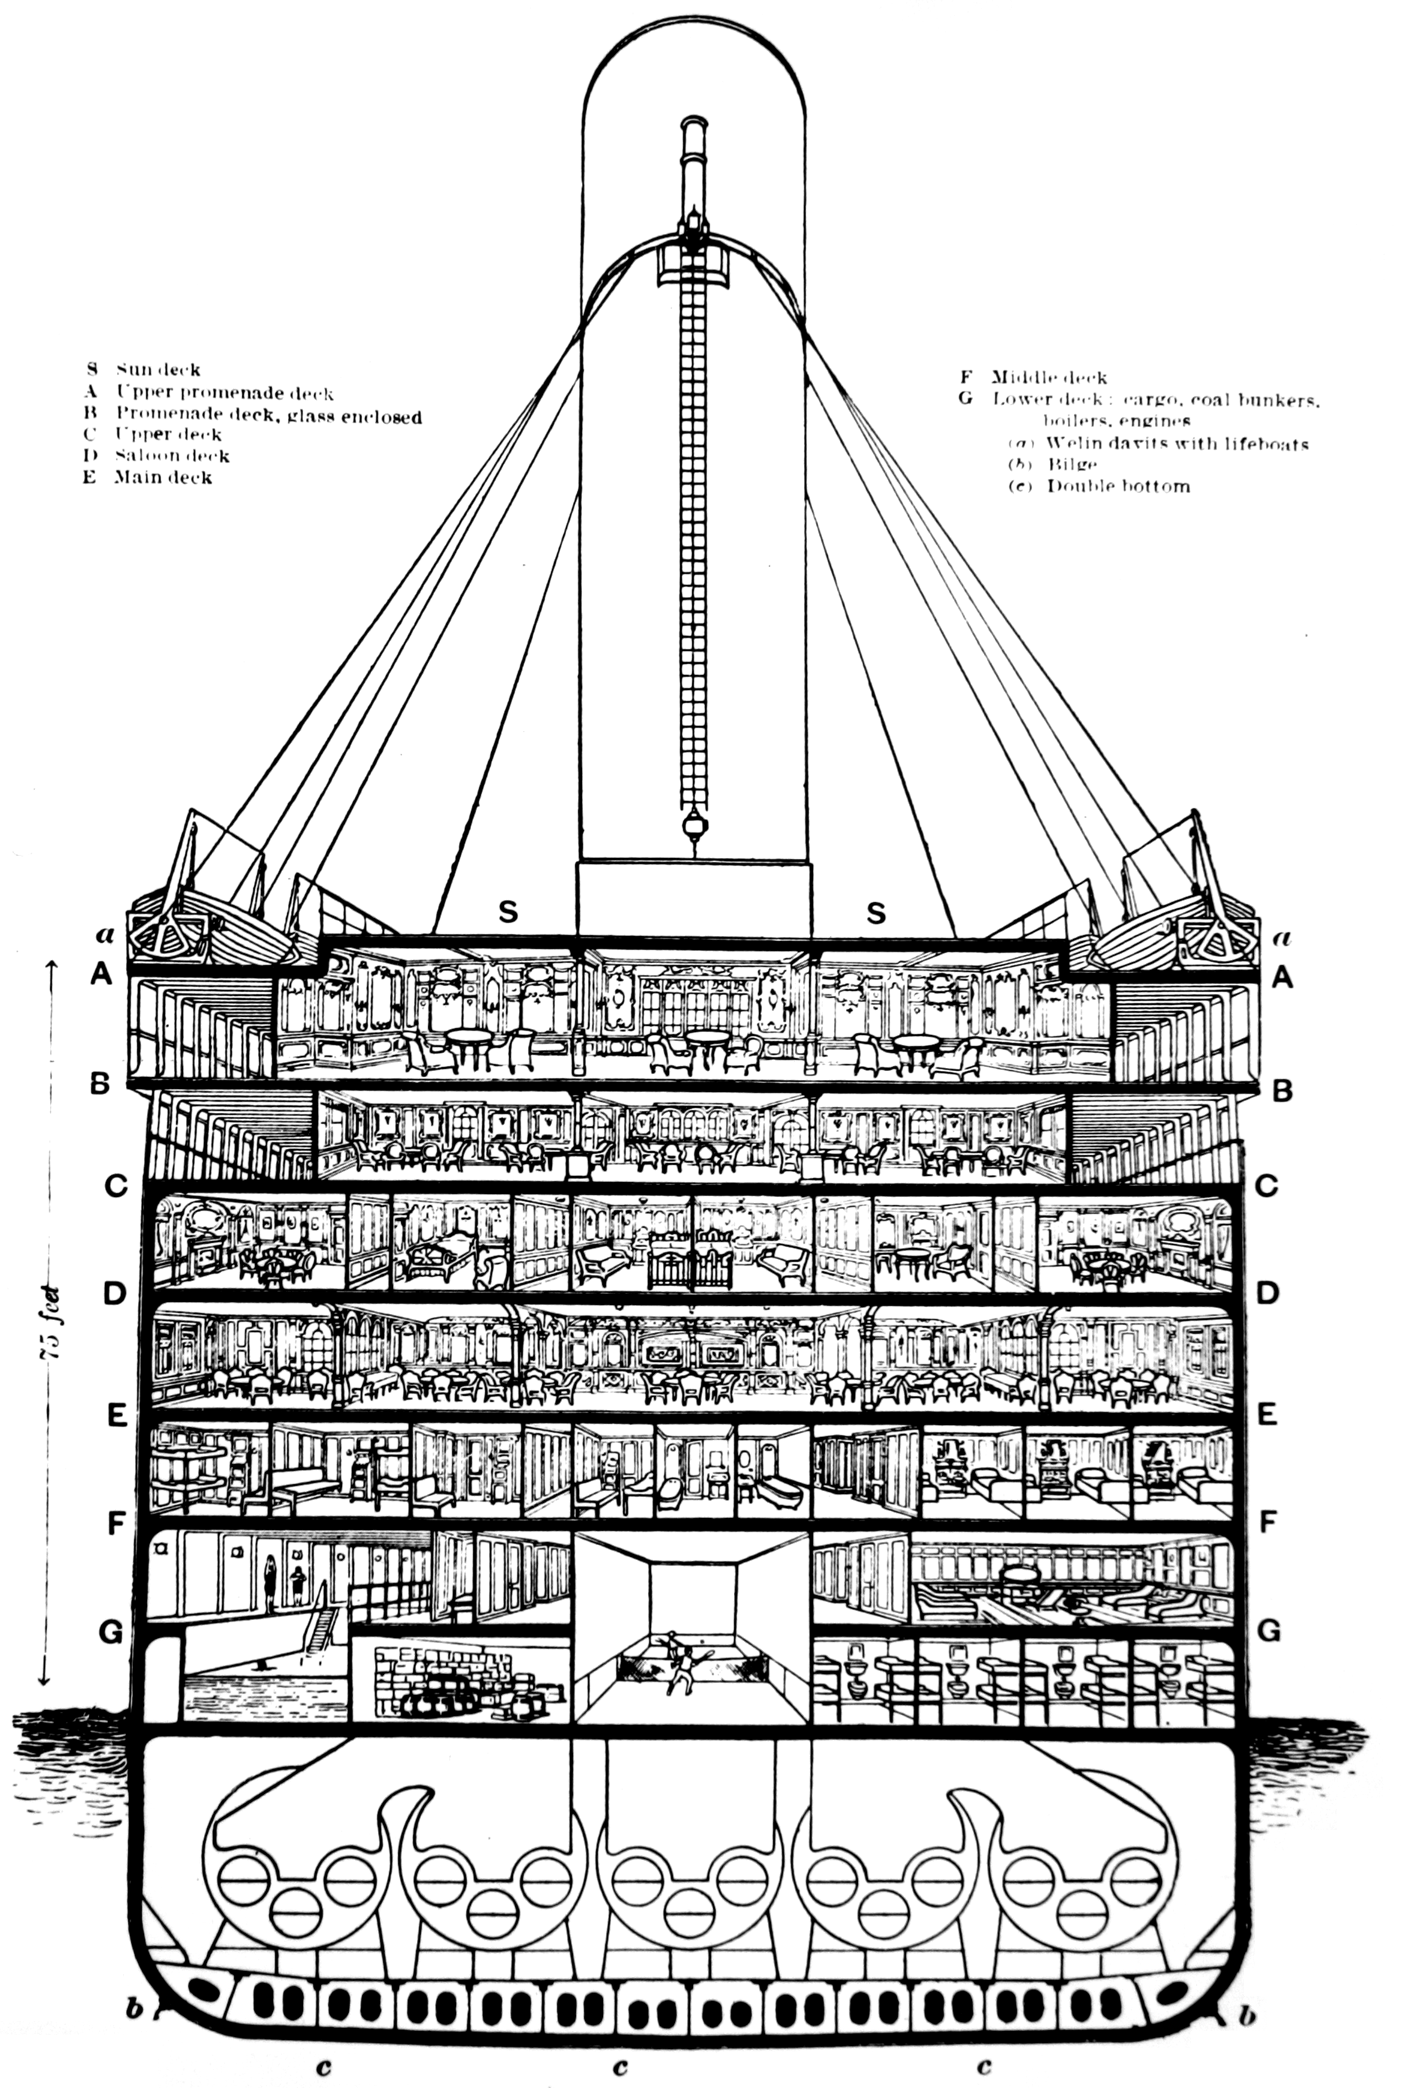
\includegraphics{assets/cross_section.png}
\caption{\label{fig:crosssection}Cross Section of the Titanic}
\end{figure}

\hypertarget{data_explore}{%
\chapter{Data Exploration}\label{data_explore}}

Placeholder

\hypertarget{summary}{%
\section{Summary}\label{summary}}

\hypertarget{variable-selection}{%
\section{Variable Selection}\label{variable-selection}}

\hypertarget{data-preparation}{%
\section{Data Preparation}\label{data-preparation}}

\hypertarget{final-data-set-summary}{%
\section{Final Data Set Summary}\label{final-data-set-summary}}

\hypertarget{correlation-investigation}{%
\section{Correlation Investigation}\label{correlation-investigation}}

\hypertarget{method}{%
\chapter{Methodology}\label{method}}

Placeholder

\hypertarget{backward-selection}{%
\section{Backward Selection}\label{backward-selection}}

\hypertarget{logistic-regression}{%
\section{Logistic Regression}\label{logistic-regression}}

\hypertarget{homser-lemeshow-goodness-of-fit-test}{%
\section{Homser-Lemeshow goodness-of-fit
test}\label{homser-lemeshow-goodness-of-fit-test}}

\hypertarget{akaike-information-criterion-aic}{%
\section{Akaike Information Criterion
(AIC)}\label{akaike-information-criterion-aic}}

\hypertarget{model}{%
\chapter{Model}\label{model}}

Placeholder

\hypertarget{model-obtained-using-backward-selection}{%
\section{Model obtained using backward
selection}\label{model-obtained-using-backward-selection}}

\hypertarget{the-final-models}{%
\section{The Final Models}\label{the-final-models}}

\hypertarget{conclusion}{%
\chapter{Conclusion}\label{conclusion}}

Placeholder

\hypertarget{findings}{%
\section{Findings}\label{findings}}

\hypertarget{further-study}{%
\section{Further Study}\label{further-study}}

\bibliography{book.bib,packages.bib}

\end{document}
